\documentclass[a4paper,14pt]{extarticle}
%\documentclass[12pt, a4paper]{article}

\usepackage[utf8]{inputenc}
\usepackage[russian]{babel}
\usepackage[left=2cm,right=2cm,
    top=1cm,bottom=2cm,bindingoffset=0cm]{geometry}
    \usepackage{graphicx}%пакет для вставки изображений
    %\graphicspath{{piсs/}}%указываем откуда следует вставлять изображения
\DeclareGraphicsExtensions{.pdf,.png,.jpg}%какое расширение будем использовать 
%\usepackage{fullpage}


\begin{document}
\newlength{\mytextsize} % определяем высоту шрифта
\makeatletter
\setlength{\mytextsize}{\f@size pt}
\makeatother
\author{Буданцев Артем}

\begin{titlepage} %Титульник

\begin{center}
{\large МИНИСТЕРСТВО НАУКИ И ВЫСШЕГО ОБРАЗОВАНИЯ РОССИЙСКОЙ ФЕДЕРАЦИИ}\\

{\small Федеральное государственное бюджетное образовательное учреждение высшего образования
«Кемеровский государственный университет»
Институт фундаментальных наук
Кафедра ЮНЕСКО по информационным вычислительным технологиям
} \\
\vspace{2cm}
{\LARGE \textbf{Отчет}}\\
по учебной практике, технологической (проектно-технологической) практике
\vspace{0.5cm}


{\large проект ``Инструменты для оформления научных статей и презентаций на примере \LaTeX'}

\vspace{4cm}

\begin{flushleft}
\textbf{Выполнили:}
\end{flushleft}
студенты направления подготовки 02.03.03 Математическое обеспечение и администрирование информационных систем 
\end{center}

\begin{flushright}
\begin{tabular}{lp{1pt}l} 
    Басалаев Дмитрий && \hspace{2cm} \\\cline{1-1}\cline{3-3} 
     {\tiny Ф.И.О.}     && {\tiny Оценка}
  \end{tabular}
  
  \begin{tabular}{lp{1pt}l} 
    Болковая Полина && \hspace{2cm} \\\cline{1-1}\cline{3-3} 
     {\tiny Ф.И.О.}     && {\tiny Оценка}
  \end{tabular}
  
   \begin{tabular}{lp{1pt}l} 
    Буданцев Артём && \hspace{2cm} \\\cline{1-1}\cline{3-3} 
      {\tiny Ф.И.О.}     && {\tiny Оценка} 
  \end{tabular}
\end{flushright}

\vspace{6cm}
\begin{center}
{\Large Кемерово 2021}
\end{center}
\end{titlepage}

\newpage%Содержание
\tableofcontents


\newpage%Првая глава
\section{``Описание проекта'}
Краткое описание: Составить презентацию и отчет о проделанной работе при помощи \LaTeX, задействовав как можно больше его возможностей.Возможно подготовить небольшую справку по интерфейсу \TeX maker.
\subsection{Актуальность, теоретическая и практическая значимость}
\textbf{Актуальность:}
Издательский пакет LateX позволяет качественно оформить любой документ или презентацию, не задумываясь о её внешнем виде, а лишь сосредоточившись на изложении и структуре. С его помощью можно легко подготовить любой документ, начиная от доклада или объемного конспекта до семестровой или курсовой работы с многочисленными формулами.
\subsection{Теоритеская значимость}
\begin{itemize}
  \item Знакомоство студентов с издательским пакетом \LaTeX, описание его примуществ и недостатков
  \item Обзор интерфейса наиболее популярного \TeX редактора ``\TeX maker'.
 \item Получение нами умения создать качественные pdf документов 
\end{itemize} 
\section{Состав группы участников проекта}
\subsection{Состав группы}
\begin{tabular}{| l| l| l| l|}
\hline {\bfseries \large №} & {\bfseries \large ФИО} & {\bfseries \large \textsl{группа}} & {\bfseries \large Логин на github.com } \\ \hline
1. & Басалаев Д.А.  & МОА-205 & FySyZe \\ \hline
2. & Болковая П.А.  & МОА-205 & ApollinariaB \\ \hline
3. & Буданцев А.А.  & МОА-205 & Antur1um \\ \hline
\end{tabular}
\subsection{Общие цель и задачи}
\textbf{Цель:} Составить презентацию и отчет о проделанной работе при помощи LateX, задействовав как можно больше его возможностей.Возможно подготовить небольшую справку по интерфейсу Texmaker.
\subsection{Распределение по ролям}
Его пока нет
\subsection{План-график работы}
\begin{tabular}{| l| l|}
\hline {\bfseries \large Даты} & {\bfseries \large Действия}\\ \hline
03.02.21-11.03.21. & Изучение базы, установка необходимого софта,подготовка документации\\ \hline
12.03.21-26.03.21 & Изучение интерфейса в \TeX maker, набор простых текстов, спецсимволы \\ \hline
27.03.21-15.04.21 & Ввод математических формул, ввод матриц,спецсимволы  \\ \hline
16.04.21-28.04.21 & Работа с ссылками,разметка страницы, различные окружения \\ \hline
29.04.21-14.05.21 & Работа с изображениями и встроенной графикой \\ \hline
15.05.21- & Разработка финального продукта, подготовка отчета. \\ \hline
\end{tabular}
\subsection{Что такое \TeX и \LaTeX ?}
\textbf{\TeX} — издательская система, созданная американским математиком и программистом Дональдом Кнутом (Donald E. Knuth). TEX был разработан преследуя две основные цели: - позволить всем создавать качественные публикации с разумными для этого усилиями. \TeX знаменит своей чрезвычайной стабильностью, работой на различных операционных системах и практически полным отсутствием ошибок. Одна из главных причин по которой \TeX выбирают для оформления научных работ заключается в том, что с его помощью можно достаточно легко вводить сложные формулы.\\

\textbf{\LaTeX} — наиболее популярный набор макрорасширений (или макропакет) системы компьютерной вёрстки \TeX, который облегчает набор сложных документов.Первая версия \LaTeX была написана в 1984 году Лесли Лампортом (Leslie Lamport) и с тех пор стала доминирующим способом подготовки \TeX публикаций. Важно заметить, что ни один из макропакетов для \TeX ’а не может расширить \TeX ’овских возможностей (всё, что можно сделать в LaTeX’е, можно сделать и в \TeX ’е), но, благодаря различным упрощениям, использование макропакетов зачастую позволяет избежать весьма изощрённого программирования.Пакет позволяет автоматизировать многие задачи набора текста и подготовки статей, включая набор текста на нескольких языках, нумерацию разделов и формул, перекрёстные ссылки, размещение иллюстраций и таблиц на странице, ведение библиографии и др. Кроме базового набора существует множество пакетов расширения \LaTeX.

\subsection{Используемые порограмные средства}
\begin{itemize}
\item[1.]Github

\item[2.]\TeX Live

\item[3.]\TeX maker
\end{itemize}
Для того чтобы использовать \LaTeX на современном ПК под управлением Windows 10 нам понадобится загрузить и установить \TeX live maneger(это наиболее полный дистрибутив \LaTeX), а также \TeX maker(это редактор для создания TEX документов). А для сохранения документов в формате pdf нам понадобится написать пару строк в командной строке.

\subsection{Что представляет собой \LaTeX докумет}
\LaTeX документ состоит из двух частей: файл с расширением .tex в котором содержатся обычный текст и команды \LaTeX(входной файл) и собственно скомпилированный pdf файл(выходной файл). Для того чтобы получить pdf файл из .tex файла нам необходимо зайти в командную строку, затем при помощи команды "cd" перейти в директорию в которой лежит .tex файл затем написать команду "pdflatex" и название файла с указанием расширения (.tex).(например: pdflatex FinalReport.tex)

\section{Ход работы}

\subsection{03.02.21-11.03.21}
Загрузили \TeX live maneger и \TeX maker. Ознакомились с интерфейсом, синтаксисом набора команд и структурой документа. Подготовили документацию по проекту.

\subsection{12.03.21-26.03.21}
Изучили набор команд для написания спец. символов и изменения шрифта(\{ \textbf{жирный}, \textsl{Курсив}, {\tiny крошечный} {\Huge Огромный} \} \$ \texteuro \   и др.)
Решили составить таблицу, содержащую наиболее часто используемые команды, но вскоре отказались от этой идеи ибо в \TeX maker присутствуют автоматические подсказки, а также многие действия вынеcены на кнопки интерфейса. 

\begin{figure}[h]
\setlength{\fboxsep}{0pt}%
\setlength{\fboxrule}{1pt}%ширина рамки
\fbox{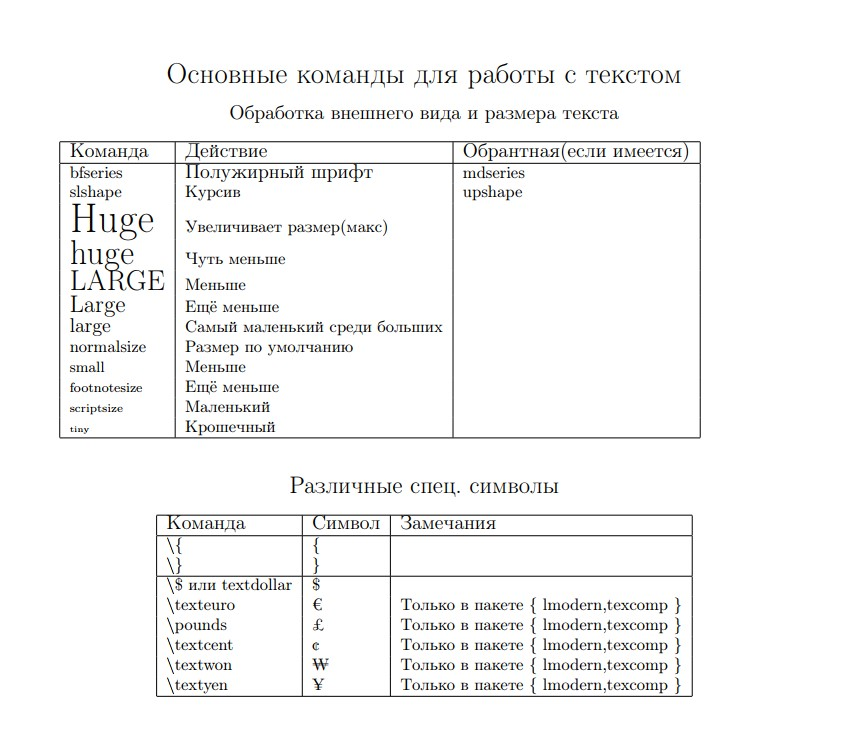
\includegraphics{table}}%
\caption{Та самая недоделанная таблица}
\label{fig:image}
\end{figure}

\newpage
\begin{figure}[ht]
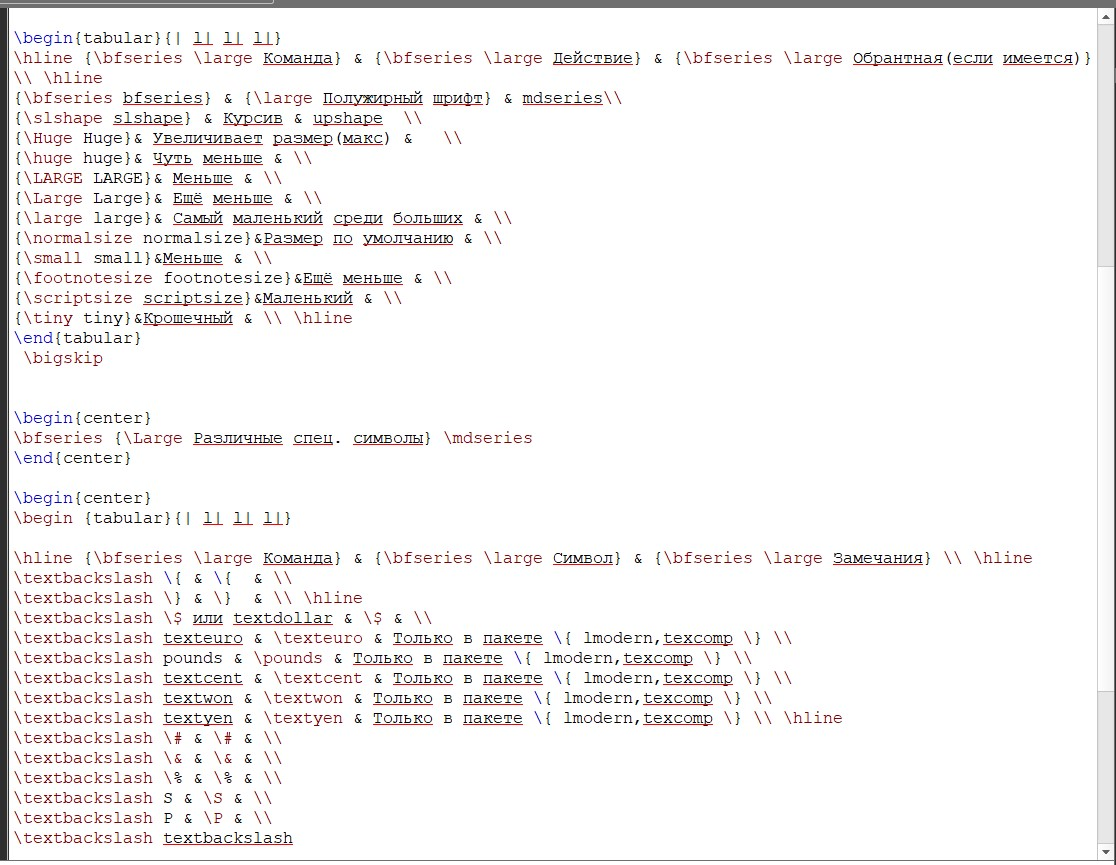
\includegraphics[width = 18cm]{TableCode}
\caption{А вот так она выглядит в \TeX maker'e }
\label{fig:image}
\end{figure}

\subsection{27.03.21-15.04.21}
Итак, мы приступили к вводу математических выражений и формул. Желая начать с чего-то простого мы решили преписать школьную таблицу производных и интегралов.





















\end{document}
